The Smartbin hardware platform is a simple construction consisting of two sensors, a microprocessor and a wifi communication module. It is embedded into a thrashbin with a lid which is used
as a base for both the distance sensor and the gas sensor.

We built the prototype using an Arduino Uno board (figure \ref{fig:board}).
 As for the sensors we used a Figaro TGS2602 as our gas sensor and a MaxSonar MB1013 ultrasonic rangefinder as our distance sensor.
We use a WiFi shield on the Arduino board for wireless communication.

The presentation layer works on Android 4.0 or later.

\begin{figure}
\centering
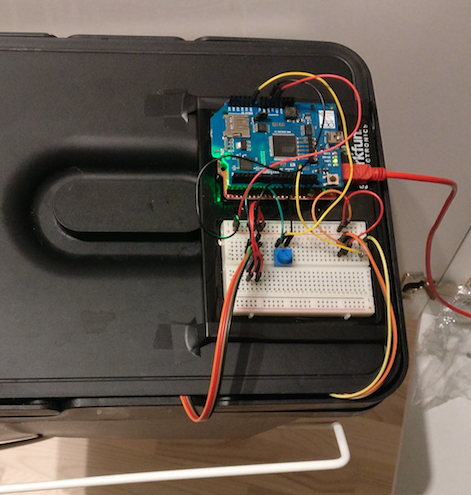
\includegraphics[scale=.3]{img/arduinoboard}
\caption{The controller board with communication shield}
\label{fig:board}
\end{figure}